

\chapter{Basics of State Space}\label{BasicsStateSpaceChapter}


\section{Problem Statement and Learning Objectives}

Most of this course will cover control system design using system transfer functions (rational polynomials in $s$ which describe the input-output relationships of system blocks).  However when we write the equations of motion, it is an ideal time to introduce a couple of concepts from the ``modern control theory" introduced in the 1960's which has supplanted the $s$ domain methods in some applications.

\paragraph{Learning Objectives}
Be able to
\begin{itemize}
    \item Understand the basic system equations to represent a linear
    dynamic system in state space.
    \item Convert equations of motion (EOMs) into state space
    representation.
    \item Use the computer to plot step response and state trajectories from
    the state space model.
\end{itemize}

\section{Introduction}
In ``modern" control theory, the system is represented as a first order linear differential equation in a high dimensional space known as state space.  Each point in state space represents a unique dynamical state of the system.   For example, a system with one mass could be described by a 2-dimensional state space consisting of the position, $x$ and the velocity, $\dot{x}$ (Figure \ref{2Dstatespace}).

\begin{figure}\centering
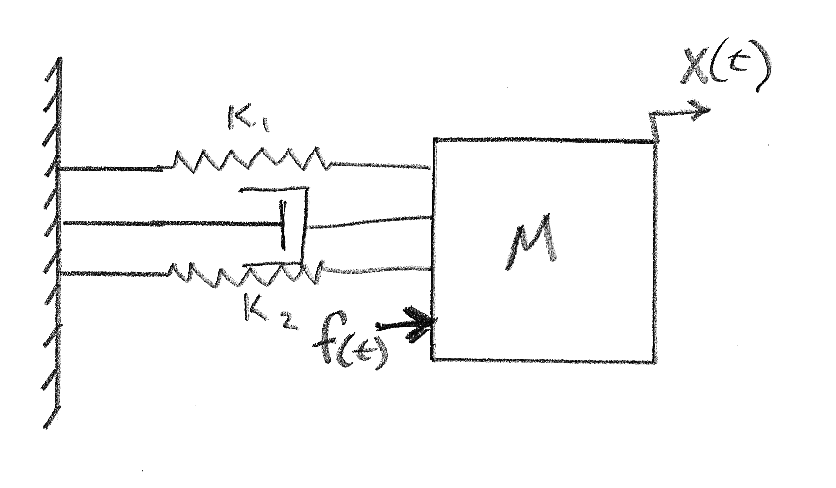
\includegraphics[width=65mm]{figs04/01069.png}   \hspace{0.25in}
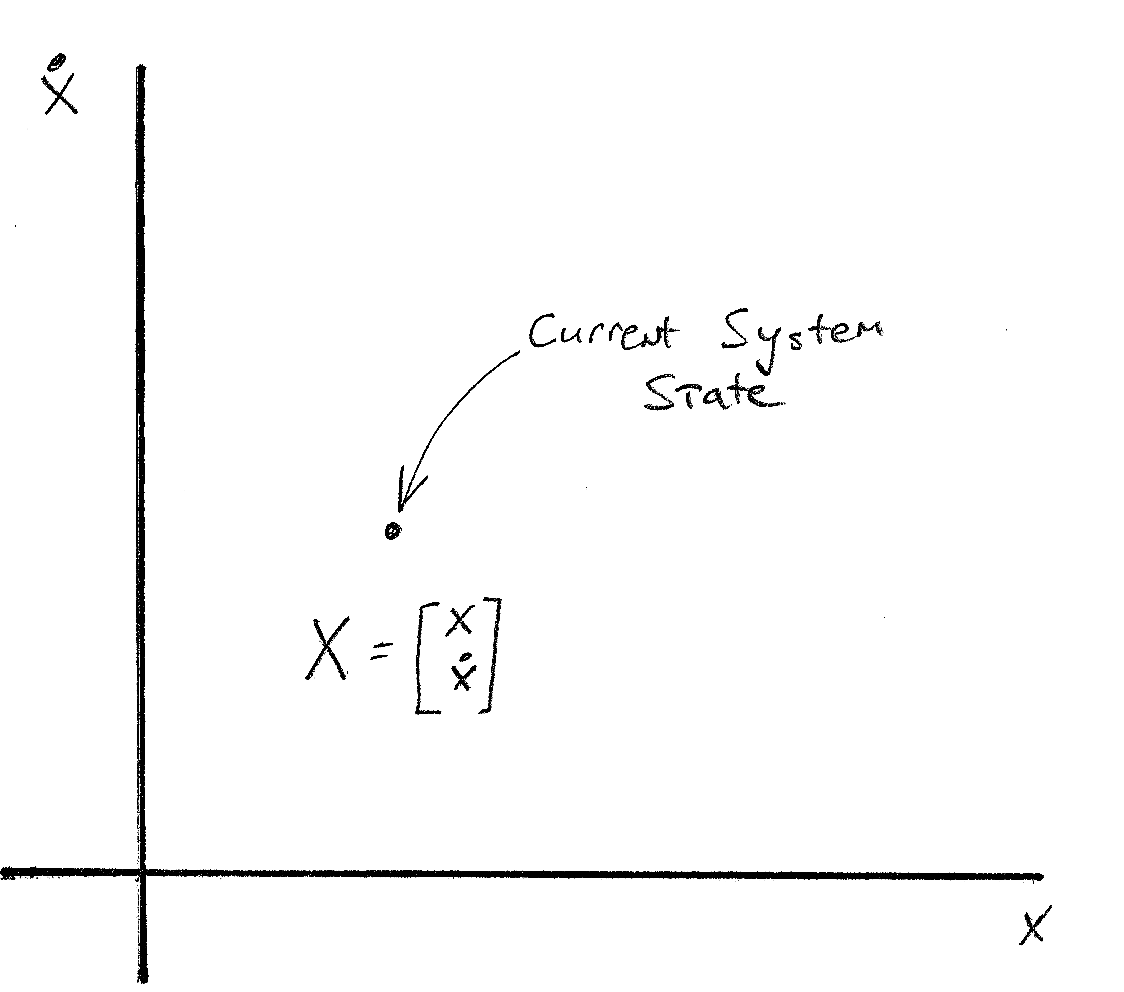
\includegraphics[width=45mm]{figs04/01075.png}
\caption{Translational dynamic system for state space example.}\label{2Dstatespace}
\end{figure}

One way to define the dimensionality of a system's state space is to identify all system variables which describe an energy.  Each one is a dimension of state space.   In our single mass example, energy is stored in the spring and mass:
\[
E_K = \frac{1}{2}(K_1 + K_2)x^2 \qquad E_M = \frac{1}{2}M{\dot{x}}^2
\]
So for this system we would use $x$ and $\dot{x}$ as state variables.
We use a vector, $X$, to define a point in state space such as:
\[
X = \begin{bmatrix} x \\ \dot{x} \end{bmatrix}
\]
Then the dynamics of the system are represented in a matrix first order LODE:
\[
\dot{X} = AX+BU
\]
Where $X$ is the state vector, $\dot{X}$ is the first derivative of the state vector,
\[
\dot{X} = \begin{bmatrix}\dot{x} \\ \ddot{x} \end{bmatrix}
\]
$A$ is a matrix of constant coefficients,
$U$ is the system input (like an applied force, $f(t)$), and
$B$ is another matrix.  This form can represent systems with multiple inputs (the elements of $U$), but here we will restrict ourselves to a single input so only one element of $U$ is non-zero.

Sometimes the output of the system, $Y$, is not one of the state variables, but instead a linear
combination of the state variables and possibly the input.  In this case there is another equation
\[
Y = CX+DU
\]
where $C,D$ are additional matrices of constant coefficients.
There is no Laplace transform and the
equations come directly from the equations of motion. In many realistic systems,
many  elements of these matrices are zero.



\section{System Matrices from Equations of Motion}
Let's see how EOMs turn into the State Space representation using the example system of Figure \ref{2Dstatespace}.  Writing the EOM:
\[
M\ddot{x}+B\dot{x}+(K_1+K_2)x = f(t)
\]
rearranging to solve for $\ddot{x}$:
\[
\ddot{x} = \frac{1}{M}\left[ -B\dot{x}-(K_1+K_2)x+f(t)\right ]
\]
\[
\ddot{x} = -\frac{B}{M}\dot{x} - \frac{K_1+K_2}{M}x + \frac{1}{M}f(t)
\]
Converting this to a matrix equation is just rearranging according to
\[
       \dot{X} = \begin{bmatrix}\dot{x} \\ \ddot{x} \end{bmatrix}
\qquad      X  = \begin{bmatrix} x \\ \dot{x} \end{bmatrix}
\qquad U       = \begin{bmatrix}0\\f(t)\end{bmatrix}
\]
%  \begin{bmatrix}\end{bmatrix}
then we have
\[
\dot{X} =
\begin{bmatrix}\dot{x} \\ \ddot{x} \end{bmatrix} =
\begin{bmatrix}0&1\\\frac{-(K_1+K_2)}{M}&\frac{-B}{M}\end{bmatrix}
\begin{bmatrix}x\\ \dot{x}\end{bmatrix}+
\begin{bmatrix}0&0\\0&\frac{1}{M}\end{bmatrix}
\begin{bmatrix}0\\f(t)\end{bmatrix}
\]
The top row is sort of a trivial equation, and the second row is the rearranged equation of motion.
This is the state space description for the system of Figure \ref{2Dstatespace}.


\begin{Example}\label{suspensionstatespace}
Consider the car suspension
Example 2.\ref{ExampleCarSuspension} and Example 2.\ref{ExampleCarSuspensionTF}.
\vspace{0.2in}
Derive the state space representation.

The EOMs were:
\begin{align*}
&M_w\ddot{x}_2+B_s(\dot{x}_2-\dot{x}_3)+K_s(x_2-x_3)+K_t(x_2-x_1) =0 \\
&M_v\ddot{x}_3+B_s(\dot{x}_3-\dot{x}_2)+K_s(x_3-x_2) = 0
\end{align*}
Note that the input to this system is $x_1$, the displacement of the road.  We  can
re-write the EOMS to put the input on the RHS:
\begin{align*}
&M_w\ddot{x}_2+B_s(\dot{x}_2-\dot{x}_3)+K_s(x_2-x_3)+K_tx_2 = K_tx_1 \\
&M_v\ddot{x}_3+B_s(\dot{x}_3-\dot{x}_2)+K_s(x_3-x_2) = 0
\end{align*}
Let the state vector be:
\[
X = \begin{bmatrix}x_2 & \dot{x}_2 & x_3 & \dot{x}_3\end{bmatrix}^T
\]
(where T indicates transpose to make $X$ a column vector)
and its derivative is
\[
\dot{X} = \begin{bmatrix}\dot{x}_2 & \ddot{x}_2 & \dot{x}_3 & \ddot{x}_3\end{bmatrix}^T
\]
Rearranging the EOMS:

\begin{align*}
\ddot{x}_2  &= \frac{1}{M_w}\left [-(K_T+K_s)x_2-B_s\dot{x}_2+K_sx_3+B_s\dot{x}_3\right]\quad+\quad \frac{1}{M_w}K_tx_1 \\
\ddot{x}_3 &= \frac{1}{M_v}\left[+K_sx_2+B_s\dot{x}_2 -K_sx_3-B_s\dot{x}_3\right]
\end{align*}

We then have the 4x4 matrix state equations:
\[
\dot{X} = \begin{bmatrix}\dot{x}_2 \\ \ddot{x}_2 \\ \dot{x}_3 \\ \ddot{x}_3\end{bmatrix}
=
\begin{bmatrix} 0&1&0&0\\
-\frac{(K_T+K_s)}{M_w}&\frac{-B_s}{M_w}&\frac{K_s}{M_w}&\frac{B_s}{M_w}\\
0&0&0&1 \\
\frac{K_s}{M_v}&\frac{B_s}{M_v}&\frac{-K_s}{M_v}&\frac{-B_s}{M_v}\\
\end{bmatrix}
\begin{bmatrix}x_2\\\dot{x}_2\\x_3\\\dot{x}_3 \end{bmatrix}+
\begin{bmatrix}
    0&0&0&0&\\
    0&\frac{K_t}{M_w}&0&0&\\
    0&0&0&0&\\
    0&0&0&0&\\
\end{bmatrix}
\begin{bmatrix} 0 \\x_1\\0\\ 0\end{bmatrix}
\]
Note that we have two trivial equations: rows 1 and 3:
\[
\dot{x}_2 = \dot{x}_2 \qquad \dot{x}_3 = \dot{x}_3
\]
Once your parameter values are known, you can plug them in and it is easy to evaluate the response to any input using the computer.
\end{Example}

\section{State Space in python}
The {\tt python.control} package has many functions to manipulate and study systems in state space.  In fact when you represent a transfer function in the Laplace domain in {\tt control} with the {\tt control.transferFunction(num,den)} command, it is internally converted into state space.   The following python code sets up the state equations for
Example \thechapter.\ref{suspensionstatespace}.

\begin{center}
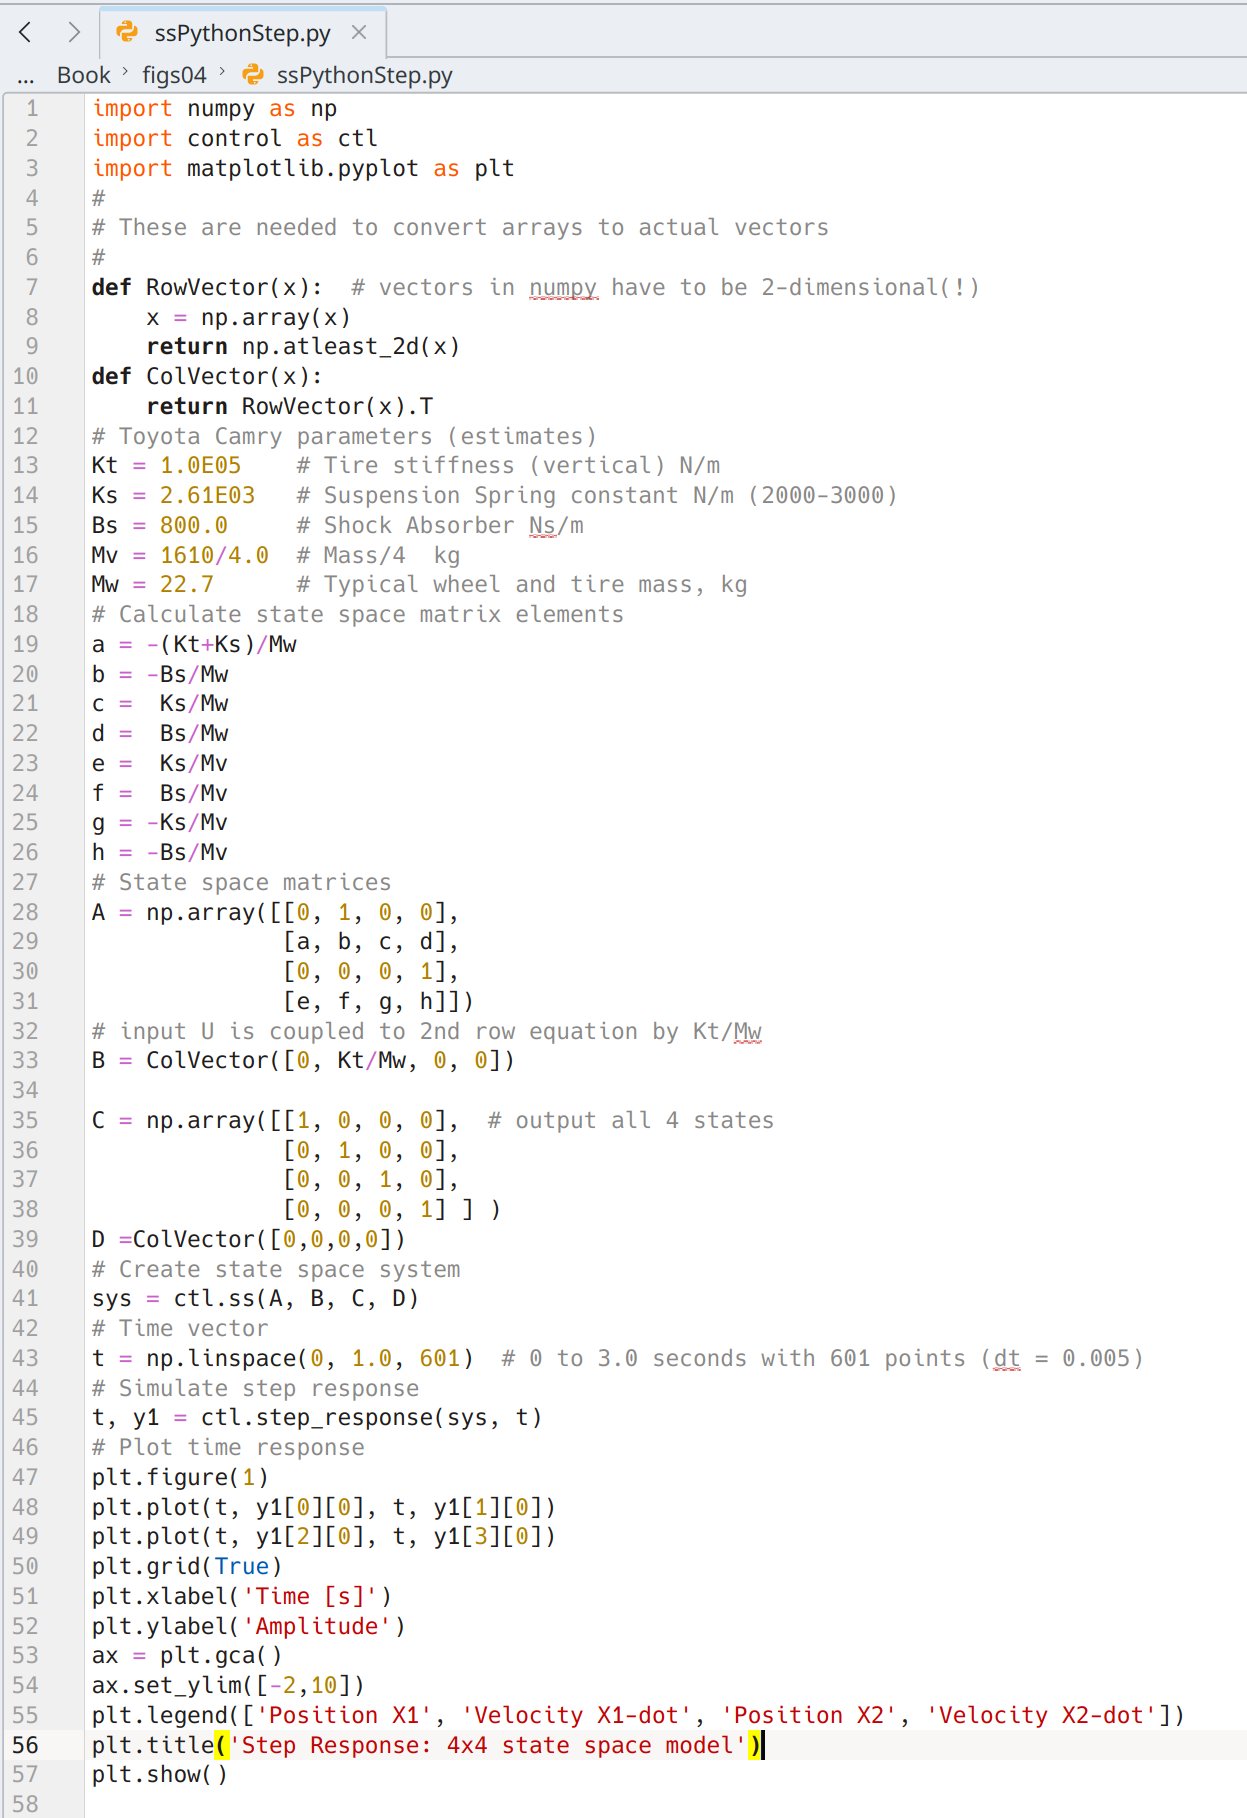
\includegraphics[width=3.5in]{figs04/python_ss_stepcode.png}
\end{center}


In lines 7 to 11 we define a couple of functions to make it easier to set up ``official"
row and column vectors in numpy.

In lines 13 to 17 we enter mechanical parameters for our car suspension.

With reference to the derived state space equation, in lines 19-26 we set
up the matrix elements, and in lines 28-39 we define the $A,B,C,D$ of the
state space equations
 \[
 \dot{x} = Ax+Bu
 \]
  \[
  y = Cx + Du
  \]

Recall that $x_1$ is not a 'state' but rather an input so our state vector is:

\[
x = [x_2,\dot{x_2},x_3,\dot{x}_3]^T
 \]

Line 41 creates a {\tt control.StateSpace} class instance from our four matrices.

In lines 43 to 45 we compute the step response of our system.   Here we should be aware
that {\tt python.control} determines the number of inputs and outputs from the dimensions of
$B$ and $C$.   If $B>1$ or $C>1$, there is more than one transfer function based on the
permutations of inputs and outputs.   For our system here, $B$ has one column (line 33) so there
is just one input and $C$ is 4x4 meaning 4 outputs.

In lines 47 to 49 we plot 4 step responses based on a 4x4 $C$ matrix (line 35) which generates
an output vector containing the step responses.

First we generate a conventional step response\footnote{Using a simplified version of lines
48 and 49.} from input (road displacement $x_1$) to car body
displacement ($x_2$) (Figure \ref{graphsuspensionstep}).

\begin{figure}\centering
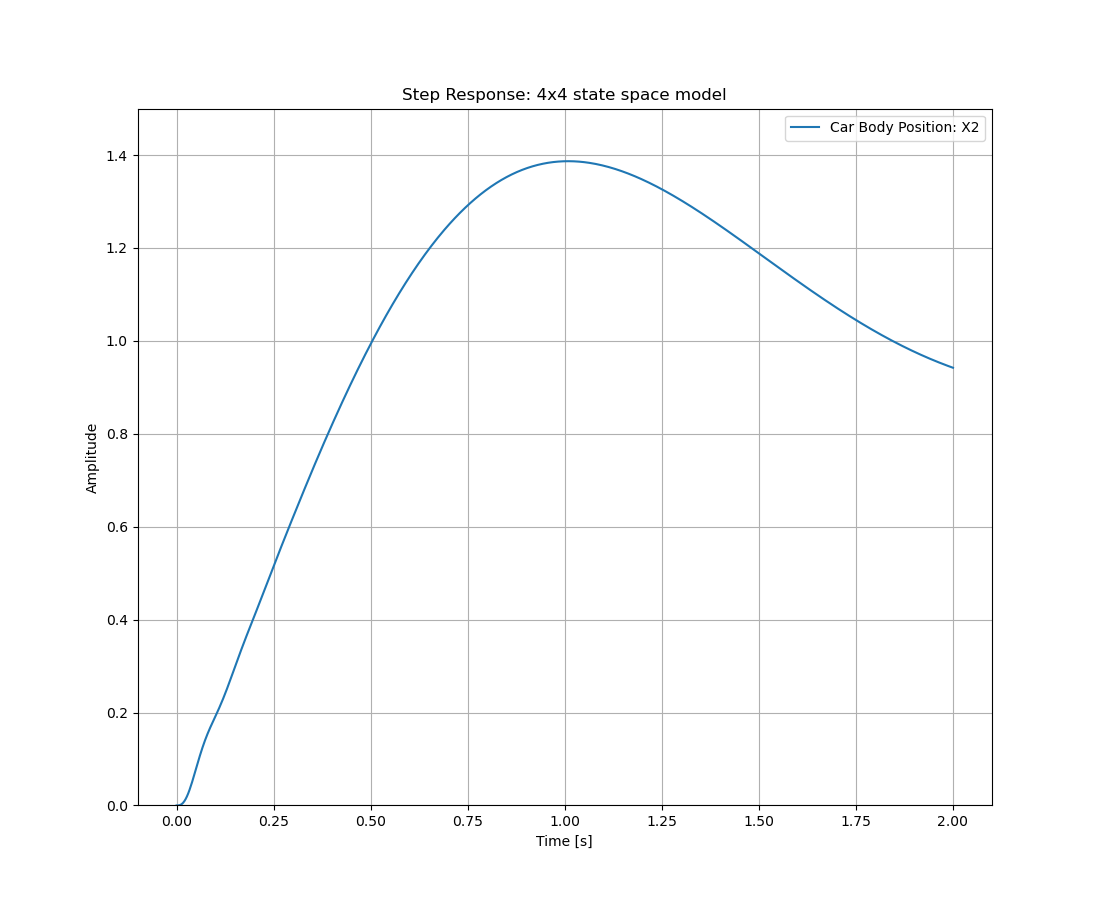
\includegraphics[width=3.5in]{figs04/singleCarBodyStep.png}
\caption{Step response of the car suspension system (overshoot indicates shocks probably
    worn out. Time for new ones!.}\label{graphsuspensionstep}
\end{figure}

Then, we can visualize all four state variables as they respond to a step input at $x_1$.

Let's visualize the step response in state space instead of the time domain.   We'll choose
a plane which is a subspace of state space: $[x_3, \dot{x}_3]$.   We add the following lines
to the script:

\begin{center}
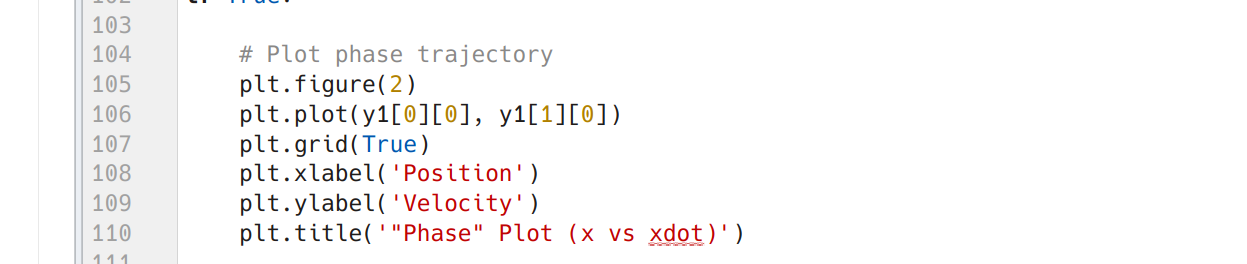
\includegraphics[width=3.5in]{figs04/ss_phase_addon.png}
\end{center}

Recall the second state space equation is
\[
y=Cx+Du
\]
to get the data for our subspace plot let
\[
C = \begin{bmatrix} 1,0,0,0 \\ 0,1,0,0 \end{bmatrix}
\]
This selects out the first two elements of $X$, $Y=[x_2, \dot{x}_2]$ (line 42,43).  Then using
the same system (lines 12-41) and simulation output (line 45),
we plot the two elements of $Y$ against each other (line 106) on a new figure.

\begin{figure}\centering
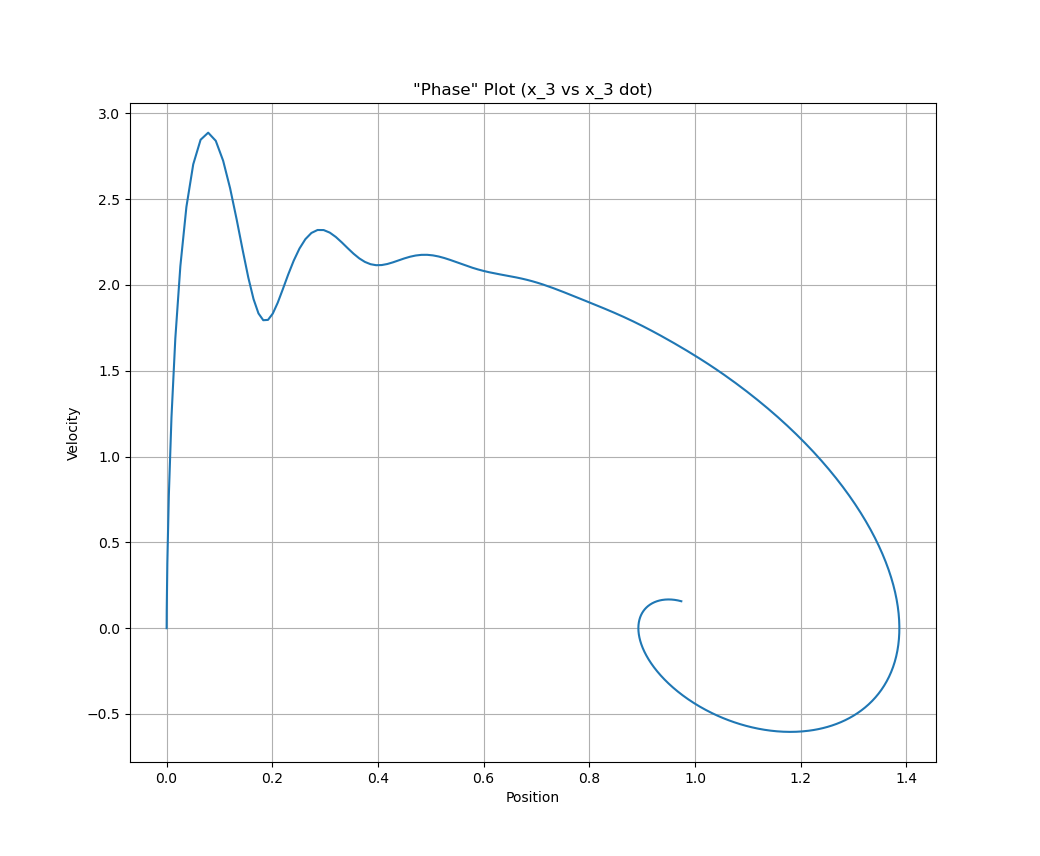
\includegraphics[width=3.5in]{figs04/py_phase_plot.png}
\caption{Step response of the car suspension system in state space.  Horizontal axis is $x_3$, the position of the car body, and vertical axis is $\dot{x}_3$, the velocity of the body's vertical travel.}\label{graphstatespacespiral}
\end{figure}

The result (Figure \ref{graphstatespacespiral}) plots the position, ($x_2$, horizontal axis) vs. velocity ($\dot{x}_2$, vertical axis).  The system trajectory is an interesting spiral from the initial point
($x_2=0, \quad \dot{x}_2=0$), to the final point ($x_2=1, \quad\dot{x}_2=0$).
The $x_2$ data is the same
as Figure \ref{graphsuspensionstep}, and the $\dot{x}$ data is its time derivative.
Time is not explicitly shown but the spiral indicates the overshoot in the step
response and its convergence to the steady state position value (1.0).

Using the state space representation we can really put the dynamic response under the microscope because the $C$ matrix let's us look at all 4 state variables after a step
input. For
\[ C = \begin{bmatrix} 1,0,0,0 \\ 0,1,0,0 \\ 0,0,1,0 \\ 0,0,0,1\end{bmatrix}
 \]
 We see the 4 step responses of all the state variables (Figure \ref{graph4steps}).

\begin{figure}\centering\label{graph4steps}
    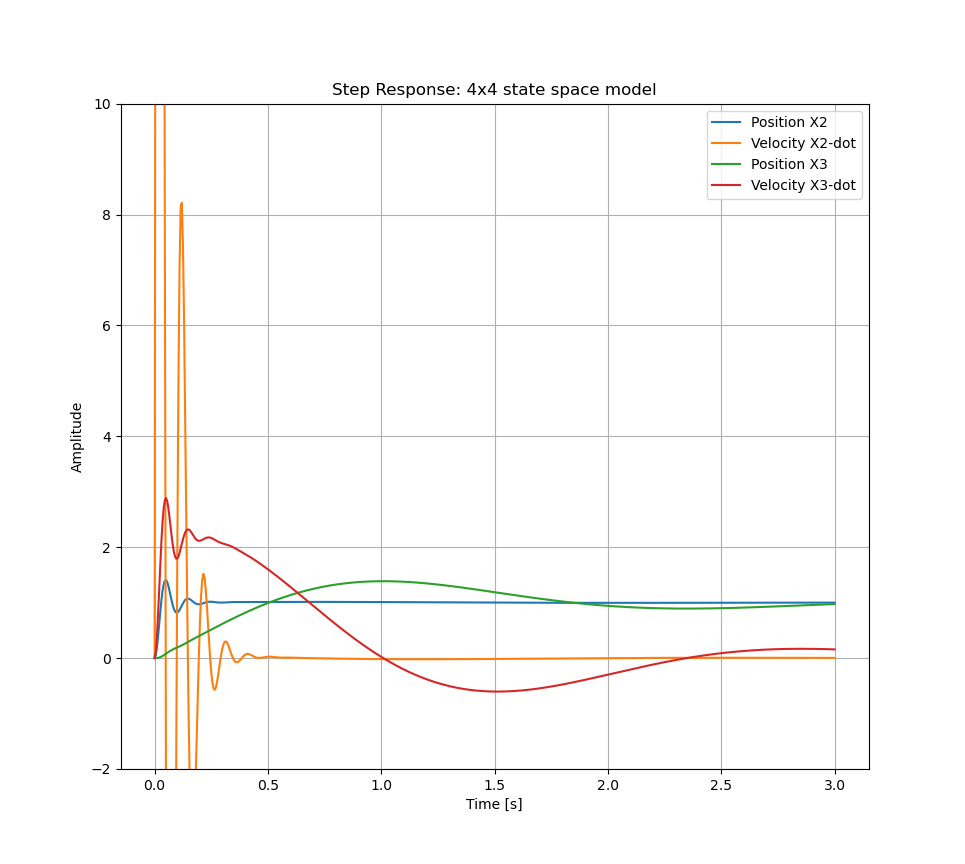
\includegraphics[width=3.5in]{figs04/all4StepResponsesCarBody.png}
    \caption{Step response of all four states of the car suspension system from the state space model. We see the car body step response (Fig \ref{graphsuspensionstep}) is now in
    green (because it is row 3).  Note change of vertical scale. }
\end{figure}

\paragraph{Converting Transfer Functions to State Space and Back}
Python control has functions to easily convert back and forth between transfer functions and state space system descriptions.   For example, suppose we have the transfer function:
\[
\frac{s+2}{s^2+20s+96}
\]
we can easily use python's {\tt tf2ss(sys)} function
to convert this to a state space representation as follows:

\begin{center}
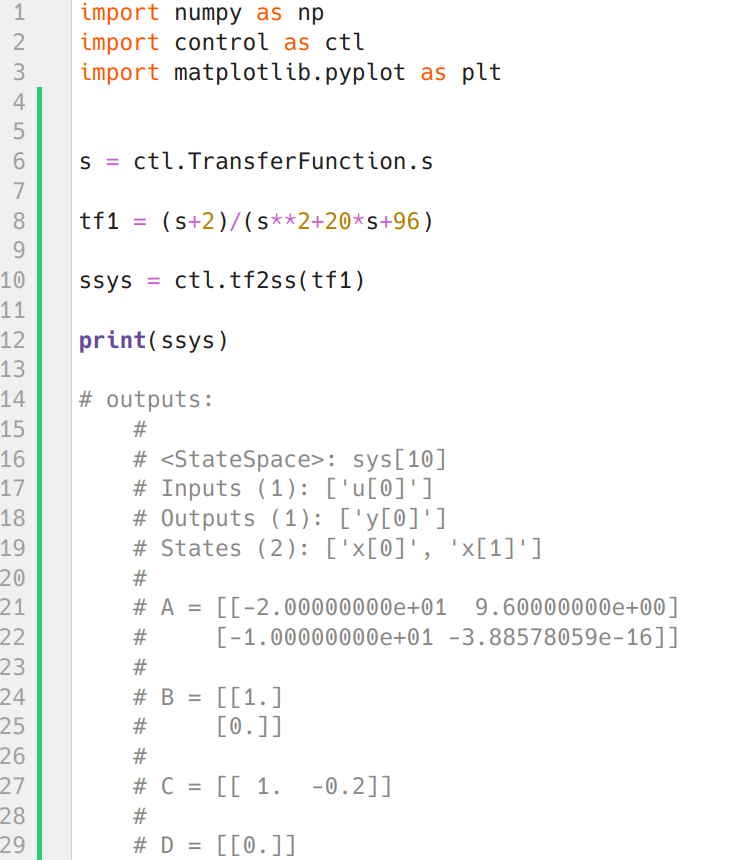
\includegraphics[width=3.5in]{figs04/Y13M75.png}
\end{center}

Python.control returns a linear system object which contains all four matrices $A,B,C,D$.
In the computation above, the matrices $A \dots D$ are not necessarily the same as those you would
derive using the system EOMs.   However they describe an equivalent dynamical system.  It turns
out there are many SS representations for each transfer function or dynamical system.
A full treatment of this issue requires a course in modern control theory, but a few interesting
 observations are worth noting.

The eigenvalues of the system matrix $A$, are the same as the poles of the transfer function.
 In the example above,

\[
\frac{s+2}{s^2+20s+96} = \frac{s+2}{(s+8)(s+12)}
\]
has poles $s=\{-8,-12\}$.    The function to compute eigenvalues in python is {\tt np.linalg.eig()}.  Using
it on the matrix $A$ computed above gives $[-8, -12]$ as expected from the poles.

%
% To see that there are infinitely many SS representations of a linear system, consider a
% rotation matrix such as
% \[
% R = \begin{bmatrix}1 & \cos{\theta} \\ -\sin{\theta} & 1\end{bmatrix}
% \]
% (such a matrix is called ``orthonormal" and has eigenvalues of unit magnitude).   The key point
% is that multiplying a matrix by a rotation matrix does not change its eigenvalues at all.   Therefore,
% if $R$ is orthonormal we can write
% \[
% RY = RAX+RBU
% \]
% and we have a new system matrix  $RA$ which represents the same system as $A$.
%


\subsection{Sources}
For Toyota Camry Suspension Parameters:
\begin{itemize}
    \item R.K. Taylor, L.L. Bashford, M.D. Schrock, ``Methods for Measuring Vertical Tire Stiffness,"
    Transactions of ASAE, vol 34, p 1415-1419, 2000
    \item M.D. Rao, S.Gruenberg, ``Measurement of Equivalent Stiffness and Damping of Shock Absorbers,"
    \item J. Iwaniec, ``Identification Of Car Suspension System Parameters On The Basis Of Exploitational Measurements," Diagnostyka, V14, N2, 2013
\end{itemize}

